% Die Arbeit besteht aus Kapiteln (chapter)
\chapter{Machinelles Lernen in der Robotik}

Die Robotik ist ein klassisches Aufgabenfeld des Machinellen Lernen. Da die durch\-zu\-führenden Aufgaben meist zu komplex sind und für diese daher keine Trainingsdaten zur Verfügung stehen, muss der Roboter durch Ausprobieren und dem daraus resultierenden Ergebnis die optimale Strategie zur Behebung des Problems finden. Durch diese Problemstellung eignet sich die Robotik insbesonders für den Einsatz von Lernen durch Verstärkung. \cite{Ertel_2013}

% Jedes Kapitel besteht aus Unterkapiteln (section)
\section{Reinforcement Learning}

Lernen durch Verstärkung, bzw. Reinforcement Learning, beschreibt ein Lernverhalten für das keine Trainingsdaten oder ähnliches vorliegen. Der Lernende bzw. Agent kann sein Verhalten nur durch Untersuchung des von der Umgebung auf eine seiner Handlungen zurückgegebenen Feedbacks optimieren. Durch das Ausführen einer Aktion wechselt, oder bleibt, der Agent in einem Zustand. Durch den nun angenommenen Zustand wird eine Belohnung definiert, die die Güte der soeben ausgeführten Aktion unter Einbeziehung des Ausgangszustandes wiederspiegelt. \cite{Ertel_2013}\par

\begin{figure}[H]
	\centering
	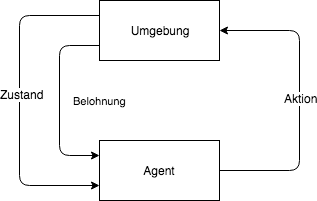
\includegraphics[width=8cm]{reinforcement-learning.png}
	\caption{Lernen durch Verstärkung}
	\label{fig:reinforcement-learning}
\end{figure}

Der Zustand $s_t \in S$ beschreibt die Umgebung des Roboters und ihn selbst zu einem bestimmten Zeitpunkt. Dies geschieht mit einer gewissen Abstraktion, da die Realität meist zu komplex ist um diese genau abzubilden und dem Agenten durch Messungenauigkeiten oder ähnliches die Informationen fehlen. Aus dem vorliegenden Zustand wird die passende Aktion $a_t \in A$ durch eine Strategie ausgewählt. Diese wird anschließend ausgeführt und die von der Umgebung zurückgelieferte Reaktion bzw. reward untersucht. Durch diesen wird die Strategie optimiert. \cite{Ertel_2013}\par
Die Strategie $\pi: S \rightarrow A$ ist optimal, wenn langfristig ein maximaler Ertrag erreicht wird. Der Wert bzw. die Belohnung der  optimale Strategie wird durch die Bewertungsfunktion 
\begin{equation}
	V^{\pi}(s_t) = \sum_{i=0}^{\infty}\gamma^{i}r_{t+1}
\end{equation}
\label{value_function_max}
beschrieben, in der direkte Belohnungen durch den Faktor $0 \le y < 1$ stärker einfließen, als weiter in der Zukunft liegende. Durch dieses kann der Agent in jedem Zustand die optimale Aktion auswählen. \cite{Ertel_2013}\par
Dies führt in der Robotik zu Problemen, da meist nicht klar ist, was für ein Zustand nach der Ausführung einer Aktion angenommen wird. Da der Wert der Strategie auf die Bewertung der Nachfolgezustände basiert kann dies nicht angewendet werden. Als Lösung hat sich das Verfahren Q-Learning etabliert, dass durch Umstellung der Gleichung \ref{value_function_max} ereicht werden kann.

\section{Q-Learning} % (fold)
\label{sec:q_learning}

Beim Q-Learning wird eine neue Bewertungsfunktion $Q(s, a)$ eingeführt. Die optimale Aktion zu einem gegebenen Zustand wird nun durch die maximale Bewertungsfunktion für den Zustand definiert. Durch Umformung der Gleichung \ref{value_function_max} wird der Wert der optimalen Bewertungsfunktion mit
\begin{equation}
	Q^{*}_t = r_t + \gamma_*Q^{*}_{t+1}
\end{equation} 
definiert. Der Wert der aktuellen Bewertungsfunktion ist sommit die Belohnung des aktuellen Zustandes und der Wert der abgeschwächten Nachfolgezustandsbewertungsfunktionen. Des Weiteren benutzt man meist noch eine Lernrate $\alpha$:
\begin{equation}
	Q(s_t, a_t) = Q(s_t, a_t) + \alpha[r_t + \gamma \ max_a Q(s_{t+1}, a_{t+1}) - Q(s_t, a_t)]
\end{equation} \cite{Ertel_2013}
Durch $\epsilon$ wird mit einer gewissen Wahrscheinlichkeit nicht die optimale sondern eine zufällige Aktion ausgeführt.\par
Zu Anfang werden die Werte der Bewertungsfunktionen zufällig initialisiert. Für den aktuellen Zustand wird die Aktion mit der größten Bewertungsfunktion ausgeführt und der neue Zustand und die daraus resultierende Belohnung analysiert. Der Wert der Bewertungsfunktion $Q(a, b)$ wird aktualisiert. Anschließend wird mit dem neuen Zustand wie mit dem vorherigen Verfahren. Dies wiederholt sich bis ein Endzustand erreicht worden ist. \cite{Ertel_2013}

% section q_learning (end)